\documentclass{article}
\usepackage{graphicx}
\usepackage{xcolor}
\usepackage{titlesec}
\usepackage[colorlinks=true,linkcolor=black]{hyperref}
\titleformat{\section}[block]{\color{blue}\Large\bfseries\filcenter}{}{1em}{}

\title{COP290 Lab 2- MyDropBox\\
	Pitara}
\date{20/2/2015}
\author{Akash Tanwar\\
		2013CS10204
		 \and
		 Aayush Gautam\\
		 2013CS10201
		 \and
		 Vivek Kumar\\
		 2013CS10263
	   }
\begin{document}
	\maketitle
	\pagenumbering{gobble}
	\tableofcontents
	\addtocontents{toc}{\protect\vspace{2ex}}
	\newpage
	\pagenumbering{arabic}
	\section{Introduction}\label{intro}
	\begin{center}
	We have named our drop box as Pitara
	\end{center}
	\subsection{Purpose of this document}
	This document is intended to give a high level overview of the backend as well as the front end of Pitara. It will explain the functionalities that we will achieve and how we are going to achieve them. We will discuss the scope of our project and the features for the same. The tools we will require for it, the data structures we will implement and how the data structures will store the users data and in what form, and much more.

	\subsection{Scope of this project}
	 \emph{Goals} -- The final goal is to develop a software that gives a user abilities to safe-upload his data on our server so that even if he loses that data on his system, he still has a copy of it on our system and can download it on any system of his choice via LAN. He may choose not to download the data on his system and still save it on our system that is he may choose to keep a synced folder or manually upload data of his choice. To achieve this we have set sub-goals for ourselves and ways to achieve them and finally build what we desire. We will discuss it later in the document in section 6.
            
               \emph{Benefits} -- There are numerous amazing benefits of this project. Some of them are:- Safe keeping data, version history of files, file sharing, retrieving deleted files, etc.
	\subsection{Overview of the document}
	This document is divided between 6 sections where the \emph{first} section, as you read, is the overview of this document.
\paragraph{}The \emph{second} section will throw some light on the functionalities, contents and design of our project and set the base for the coming sections.
\paragraph{}The \emph{third} section targets the components that we have divided our structure in and how they interact with each other.
\paragraph{}The \emph{fourth} section will explain how we handle or process the user information and store them on the server and how and which data structures we will use.
\paragraph{}The \emph{fifth} section is about our GUI, another important component of our project. We will discuss how user will interact with the software.
\paragraph{}The \emph{sixth} and the last section discusses our sub-goals and the final goal that we will achieve. It discusses what improvements we will make in a stepwise fashion and how we will implement them and a discussion on all the additional features that we are going to add.
\paragraph{}The \emph{seventh} section is a `post script' type section. It tells all about the deviations from this design document finally, now that we have made the final Pitara.

	\section{System Overview}\label{sysover}
	\subsection{Functionality}
	\paragraph{1.} \emph{Sharing :} A user will have two options \emph{one} - to share a file with another user on Pitara \emph{two}- to share it with someone not on Pitara. Every file will have certain permissions that the user can change. (A subtle improvement of ours)
\paragraph{2.} \emph{Sync :} The user will have two ways of syncing data. \emph{One}- by keeping a folder in sync with it and Pitara will automatically keep it in sync or manually select a file and upload it on Pitara to download it in future so that the user doesn't need to keep that file on his system anymore.
\paragraph{3.} \emph{Minimal Data Usage :} If a user uploads a same file again then only one copy of it will be saved.
\paragraph{4.} \emph{File History : } All the files will have a history attached to them. Whenever the user updates a file then next version of that file will be saved with minimal extra space usage.
\paragraph{5.} \emph{Security :} All the data of Pitara will flow over a secure session.
\paragraph{6.} \emph{Persistent Storage :} The client will monitor the folder in pre-defined intervals of time(changeable by the user). Every time the client monitors the folder then it will spot all the changes in its files and send data to the server. This way even if the connection is lost, it won`t be a problem to keep in sync with the user.
\paragraph{7.} \emph{Additional functionalities :} The user can delete the uploaded files whenever he wishes to. These files are those which the user uploaded by will and not kept in the folder that is in `sync? with the server. 
We will also have trash folder, from where the deleted files can be retrieved.
	\subsection{Content}
	The content that the user has to be concerned about is the GUI application package. He needs to install the GUI package to set up a working Pitara on his system.(This package has all the client side code as well as the user interface) If the user has a login ID provided by us then he can access his account and start the sync process or using the application`s abilities. If he doesn`t have an account he still can download a file shared with him by a Pitara user.
The server will have its code running continuously that will be accessible only to us. The files of the user as well as the files that have data regarding those files(version history etc.) will be stored on the server.
	\subsection{Design}
	The design of GUI is done using Qt. Qt is a tool that will help us in making the desktop application for the user. For forming a connection between client and the server we will use TCP socket programming and openSSL for security. The user will have all the features available to him with a click while server will have its program up and running. With the user`s click, client side?s functions will be controlled and communication of sockets shall proceed accordingly. We will form a simple command line way to configure the server if required. As of yet we have not planned to use any other tools other than these but we might use external libraries of c++ like boost.
	\section{System Architecture}\label{sysarch}
	\begin{figure}
\centering
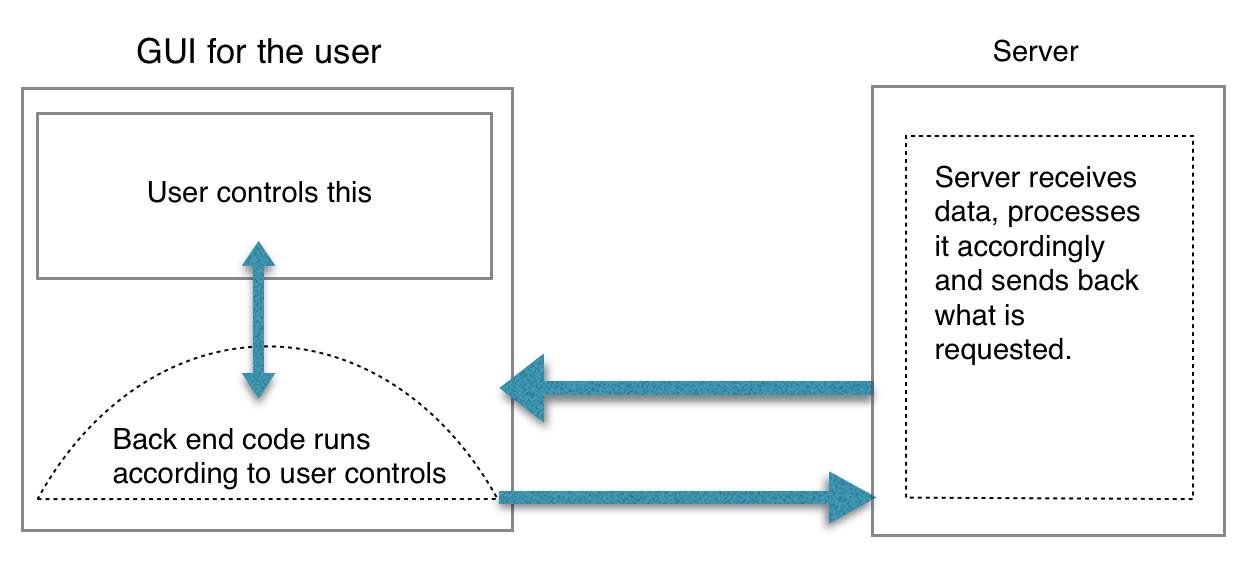
\includegraphics[width=90mm]{diagram.png} 
\caption{Project components}\label{this}
\end{figure}
	\subsection{Architectural design}
	How the project is \emph{partitioned}-- Client, server and the GUI. See Figure 1.
Their \emph{tasks}-- 
\paragraph{GUI}-- This shall be made on Qt. This will provide an easy-to-use access to all the features of Pitara. This is like the steering and gear of a car where the engine is the Client. 
The user may-- choose the files to upload, the folder to sync with, view his uploaded data, which version of a file to download, delete a file, share a file and with whom, set permissions of the file and download a shared file as well. He may also see his data limit used or ask us to increase/decrease his data limit.
\paragraph{Client}-- This is the actual engine of the GUI. When a user opens the application and logs in, the client code automatically connects with the socket of the server code which is up and running. If the login id and password are correct he will connect to the server. Now once connected, any button that the user has with him, if pressed, will carry out its function, that is the client code. 
The client will automatically monitor a folder chosen by the user and see if there was any file changed. If there is then it will automatically send it to the server as explained in the next task of the client. 
When a user chooses a file that he wants to upload, the client will access that path and start uploading that file in chunks. The chunk will have a size of 4mbs. These chunks will be sent by the client side code and received by the server(in the same order) which then will process it accordingly.
Similarly if the client wants to see what all data has been stored on the server, then client shall send an appropriate request and receive an appropriate output, and the GUI will display it. So one of the main task of the client part is to generate an appropriate request and process the received data such that the data is stored on the client?s computer or displayed by the GUI as required.
Another important task is to notice any changes done in a file on the client`s side and send appropriate request and data to the server. It shall also notice the date and time on the client`s side.

\paragraph{Server}-- The server receives requests by the client, processes it accordingly and sends the appropriate data. Server holds the key to all the data management (discussed in the next section).
When ever the client starts sending the chunks of a file, all of them will have a date with them. If the user uploads the same file again then we shall store a new chunk only if it differs from the previous chunk of the same order of the same file. If a chunk doesn`t differ then only the latest date will be added along with the previous date. If the user asks for a previous version of the same file at some other time then server will start sending back the chunks of that date in proper order. This also helps in minimal data usage. This is an overview of basic file sharing between client and the server.
Server will know all the permissions of a file that the user has set and the date of the chunks will be stored at all times, so that the storage is also persistent for the user.
Since the data is encrypted with openSSL so every `dialogue' between the client and the server is also secure.
	\subsection{Design rationale}
	The above architectural design is the best because of two main reason:-
\paragraph{1. Boldest boundaries}-- These three(GUI,client,server) are the three main aspects of this project and thus the boundaries between them are bold. This helps in easy understanding of the functioning and makes the project easy to implement.
\paragraph{2. Maximum efficiency}--
Since we have a team of 3 so splitting up the project in 3 will be fastest in this case. We can have maximum efficiency like this.
	\section{Data Design}\label{dd}
	 \subsection{Data description}
	 The data structures inside the program will mainly be arrays. The fixed size array in server will receive the chunks from the client side which will extract the data of the file in chunks with a same sized array. This will keep on happening until the whole file has been processed. Each file will be stored on the server split into chunks and not the actual file. Every file will have `.txt' corresponding to it. This file will store all the permissions, information about its chunks and versions(which date-which chunk) and any other such information if necessary.
	 
	
	 \subsection{Data rationale}
 We are using fixed size arrays in the program since it will enable us to send fixed size chunks thus helping us in splitting and joining the file,whenever necessary, easily. Also we will store the user-specific-data in `.txt' files because they are easy to use and easy to process at any time. All we need is a `naming' and a `data storing' format which shall remain fixed on the server. This will also result in no loss of data or storage even if the server stops running in between.
   \begin{figure}
\centering
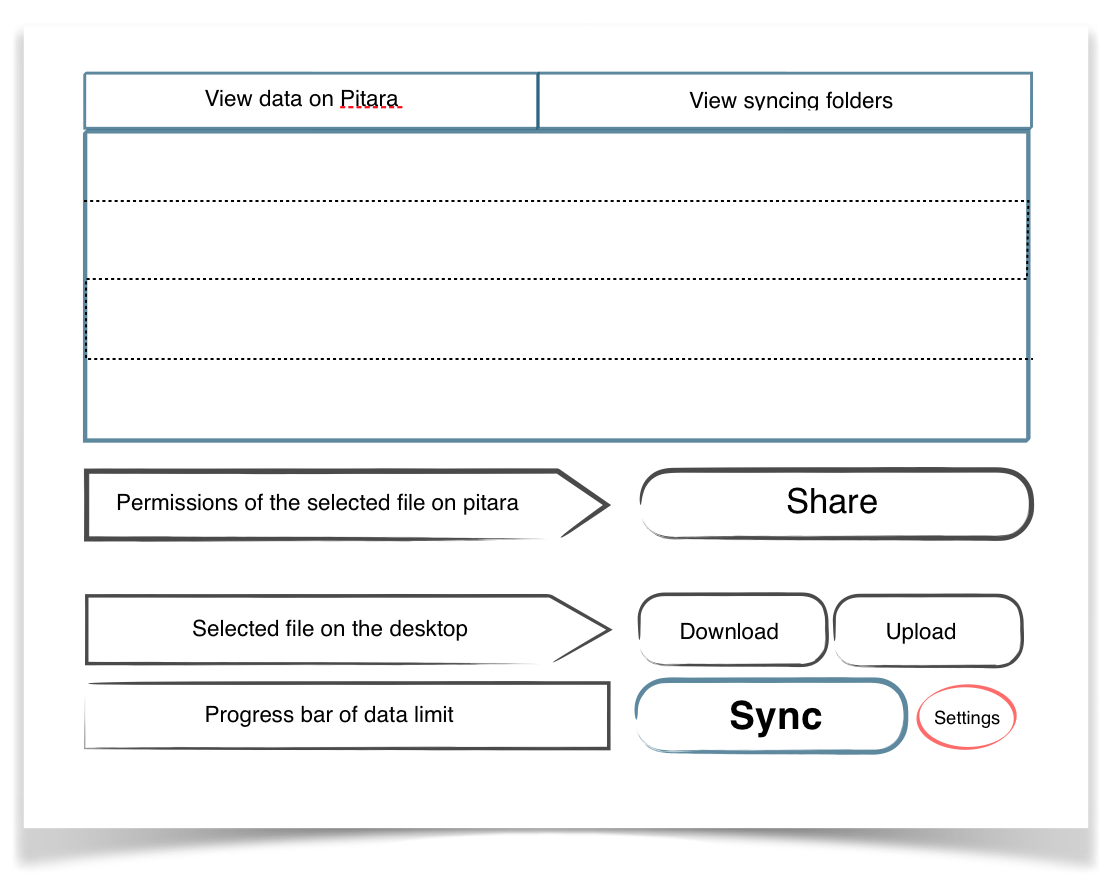
\includegraphics[width=90mm]{diagram2.png} 
\caption{GUI for the user}\label{this}
\end{figure}
 We can always start the server again and it can process the files anytime to know the user's personal information.
Also chunks help in minimal data usage and version history of a file. (as explained earlier)

	\section{Human interface design}\label{hid}
	There are only few buttons that can do a lot. There is a table on top that shows the files on Pitara or the folders that have been chosen by the user to be kept in sync with Pitara. If a file is selected from the table then the user can change its permissions and share it. When share is clicked a dialog will appear that will ask if the file has to be shared with another user of Pitara or someone who is not on Pitara. The user can select a file on his desktop and upload it or download a file. The progress bar shows the data limit of the user and how much has been used and sync button is for manually syncing the folders of the user. There is a settings button which will allow the user to select more folders, change auto-sync settings, etc.
	
	See Figure 2 for details.
	\section{Steps of implementation}\label{soi}
	\paragraph{Step  1}-- We will set up the basic GUI working with Qt, where first a login screen appears and then after login the main screen with a table of user's file on the server and upload-download functionalities will appear.
\paragraph{Step 2}-- Now we will configure the folder syncing such that the client can display the files of the user that are on the server and the client knows all the data and changes in that specific folder. (Till now only folder syncing is allowed to the user)
\paragraph{Step 3}-- We will start configuring the client and server to send and receive data, such that we can upload any file and the server stores it in chunks, and the client can download the file and save it as an original.
\paragraph{Step 4}-- Now what we need to do is configure the automatic monitoring feature. Once the client is monitoring then we can send and receive data easily and a folder sync is ready.
\paragraph{Step 5}-- Now once uploading and downloading is set up, we will add the `version-history' feature, that is attaching a date with all the chunks and writing them to the `.txt' file corresponding to that file.
\paragraph{Step 6}-- Now we will add permissions to the files that will be stored in the `.txt' file. With this we will add a share functionality in the GUI of the client that can change the permissions of a file and share it with a user on Pitara.
\paragraph{Step 7}-- After this we will improve the share feature such that a user can share the files with a person who is not on Pitara. This shall be done by giving an encoded location to the file and changing the permissions so that a person not on Pitara can use that to get access to the file by providing an option at the login screen.
\paragraph{Step 8}-- The user should be able to upload a file to the server by browsing any file on his desktop. That means now we will add the path specific uploading of a file.
\paragraph{Step 9}-- Deleting and restoring a file from the server will be provided to the client now.
\paragraph{Step 10}-- If we have time left then we will jump onto internet access. Then the user can access Pitara from the internet also and not only LAN.
\paragraph{} Following these steps we will have Pitara with us with all the additional features of ours.

\section{Deviations from the document}\label{devs}
	\subsection{Minimal data usage and Version history}
	\paragraph{}We had earlier mentioned to store a file as its chunks but we realised later on that there are two main problems in it.
	\subparagraph{1.} \emph{Too tough: }It was basically too tough to achieve since storing and comparing two files chunk wise perfectly is difficult. Most of the times the server will say that `not matching' even though they do. 
	\subparagraph{2.} \emph{A problem: } Even if we had done the chunk wise comparison then minimal data usage couldn't have been achieved. This is because the sooner the change in the new version of a file appears, the larger data we would have to store because all the chunks after that will be different. And most of the times, the change will at least be in midway.
	\subparagraph{Solution: }What we did was store the files as a whole and scrapped the idea of a chunk wise comparison. We found out how `Git' works and learned about it, the \emph{diff} and \emph{patch} but unfortunately couldn't apply them on binary files. So, when a next version comes, we save the whole file, and not just the `diff'. What we did for the minimal data usage is in sharing. When a user shares a file with another user, it is only a new `pointer' in the database of the user with which the file has been shared. Thus saving space, since there is no copying.
	\subsection{Some better features: }
	\paragraph{Sign in and Sign up }We have also given the functionality of signing in to the app and sign up for a new user. The sign up is free at the moment. Username has to be different and the user sets his own password. His ID and database is unique.
	\paragraph{Forgot password }We have also added a feature that helps a user retrieve his password by answering the security question. The answer should be same as the answer that the user gave during sign up.
	\paragraph{Design }We changed the design quite a bit, and improved a lot. Our design is very user friendly and minimal but it can do a lot.
	
\end{document}